% This must be in the first 5 lines to tell arXiv to use pdfLaTeX, which is strongly recommended.
\pdfoutput=1
% In particular, the hyperref package requires pdfLaTeX in order to break URLs across lines.

\documentclass[11pt]{article}

% Remove the "review" option to generate the final version.
% \usepackage[review]{MAIN}
\usepackage[]{MAIN}

% Standard package includes
\usepackage{times}
\usepackage{latexsym}

% For proper rendering and hyphenation of words containing Latin characters (including in bib files)
\usepackage[T1]{fontenc}
% For Vietnamese characters
% \usepackage[T5]{fontenc}
% See https://www.latex-project.org/help/documentation/encguide.pdf for other character sets

% This assumes your files are encoded as UTF8
\usepackage[utf8]{inputenc}

% This is not strictly necessary, and may be commented out.
% However, it will improve the layout of the manuscript,
% and will typically save some space.
\usepackage{microtype}

% This is also not strictly necessary, and may be commented out.
% However, it will improve the aesthetics of text in
% the typewriter font.
\usepackage{inconsolata}

% Used for including images
\usepackage{graphicx}

% Better visual effect of hyper-links
\usepackage{hyperref}
\usepackage{xcolor}
\usepackage{color}
\hypersetup{
    colorlinks,
    linkcolor={red!50!black},
    citecolor={blue!50!black},
    urlcolor={blue!80!black}
}

% Show header and footer
\usepackage{fancyhdr}

\pagestyle{fancy}
\fancyhf{} % Clear existing header and footer
\fancyfoot[C]{\thepage} % Place the page number in the center of the footer

% Math
\usepackage{amsmath}


% If the title and author information does not fit in the area allocated, uncomment the following
%
%\setlength\titlebox{<dim>}
%
% and set <dim> to something 5cm or larger.

\title{Community Detection and Analysis on DBLP v9 Dataset: Centrality, Network Metrics, and Predictive Modeling}

% Author information can be set in various styles:
% For several authors from the same institution:
% \author{
%   Author 1 \and ... \and Author n \\
%   Address line \\ ... \\ Address line
% }
% if the names do not fit well on one line use
%         Author 1 \\ {\bf Author 2} \\ ... \\ {\bf Author n} \\
% For authors from different institutions:
\author{
  Xiang Zheng \\ 21307110169 \And  
  ... 
  \vspace{0.7cm} \\ % Add some space before the school name
  \hfill School of Data Science, Fudan University \hfill
  \And
  Author n \\ Address line
}

\begin{document}
\maketitle
\begin{abstract}
	abstract
\end{abstract}

\section{Introduction}

Network analysis is a critical methodology for studying complex systems across various domains. The \href{https://www.aminer.cn/citation}{DBLP dataset}, a comprehensive bibliographic resource for computer science, forms the foundation for investigating collaboration patterns and scholarly relationships. This study applies advanced graph analysis techniques to explore the structural and functional properties of the DBLP v9 dataset.

\begin{figure}[ht]
	\centering
	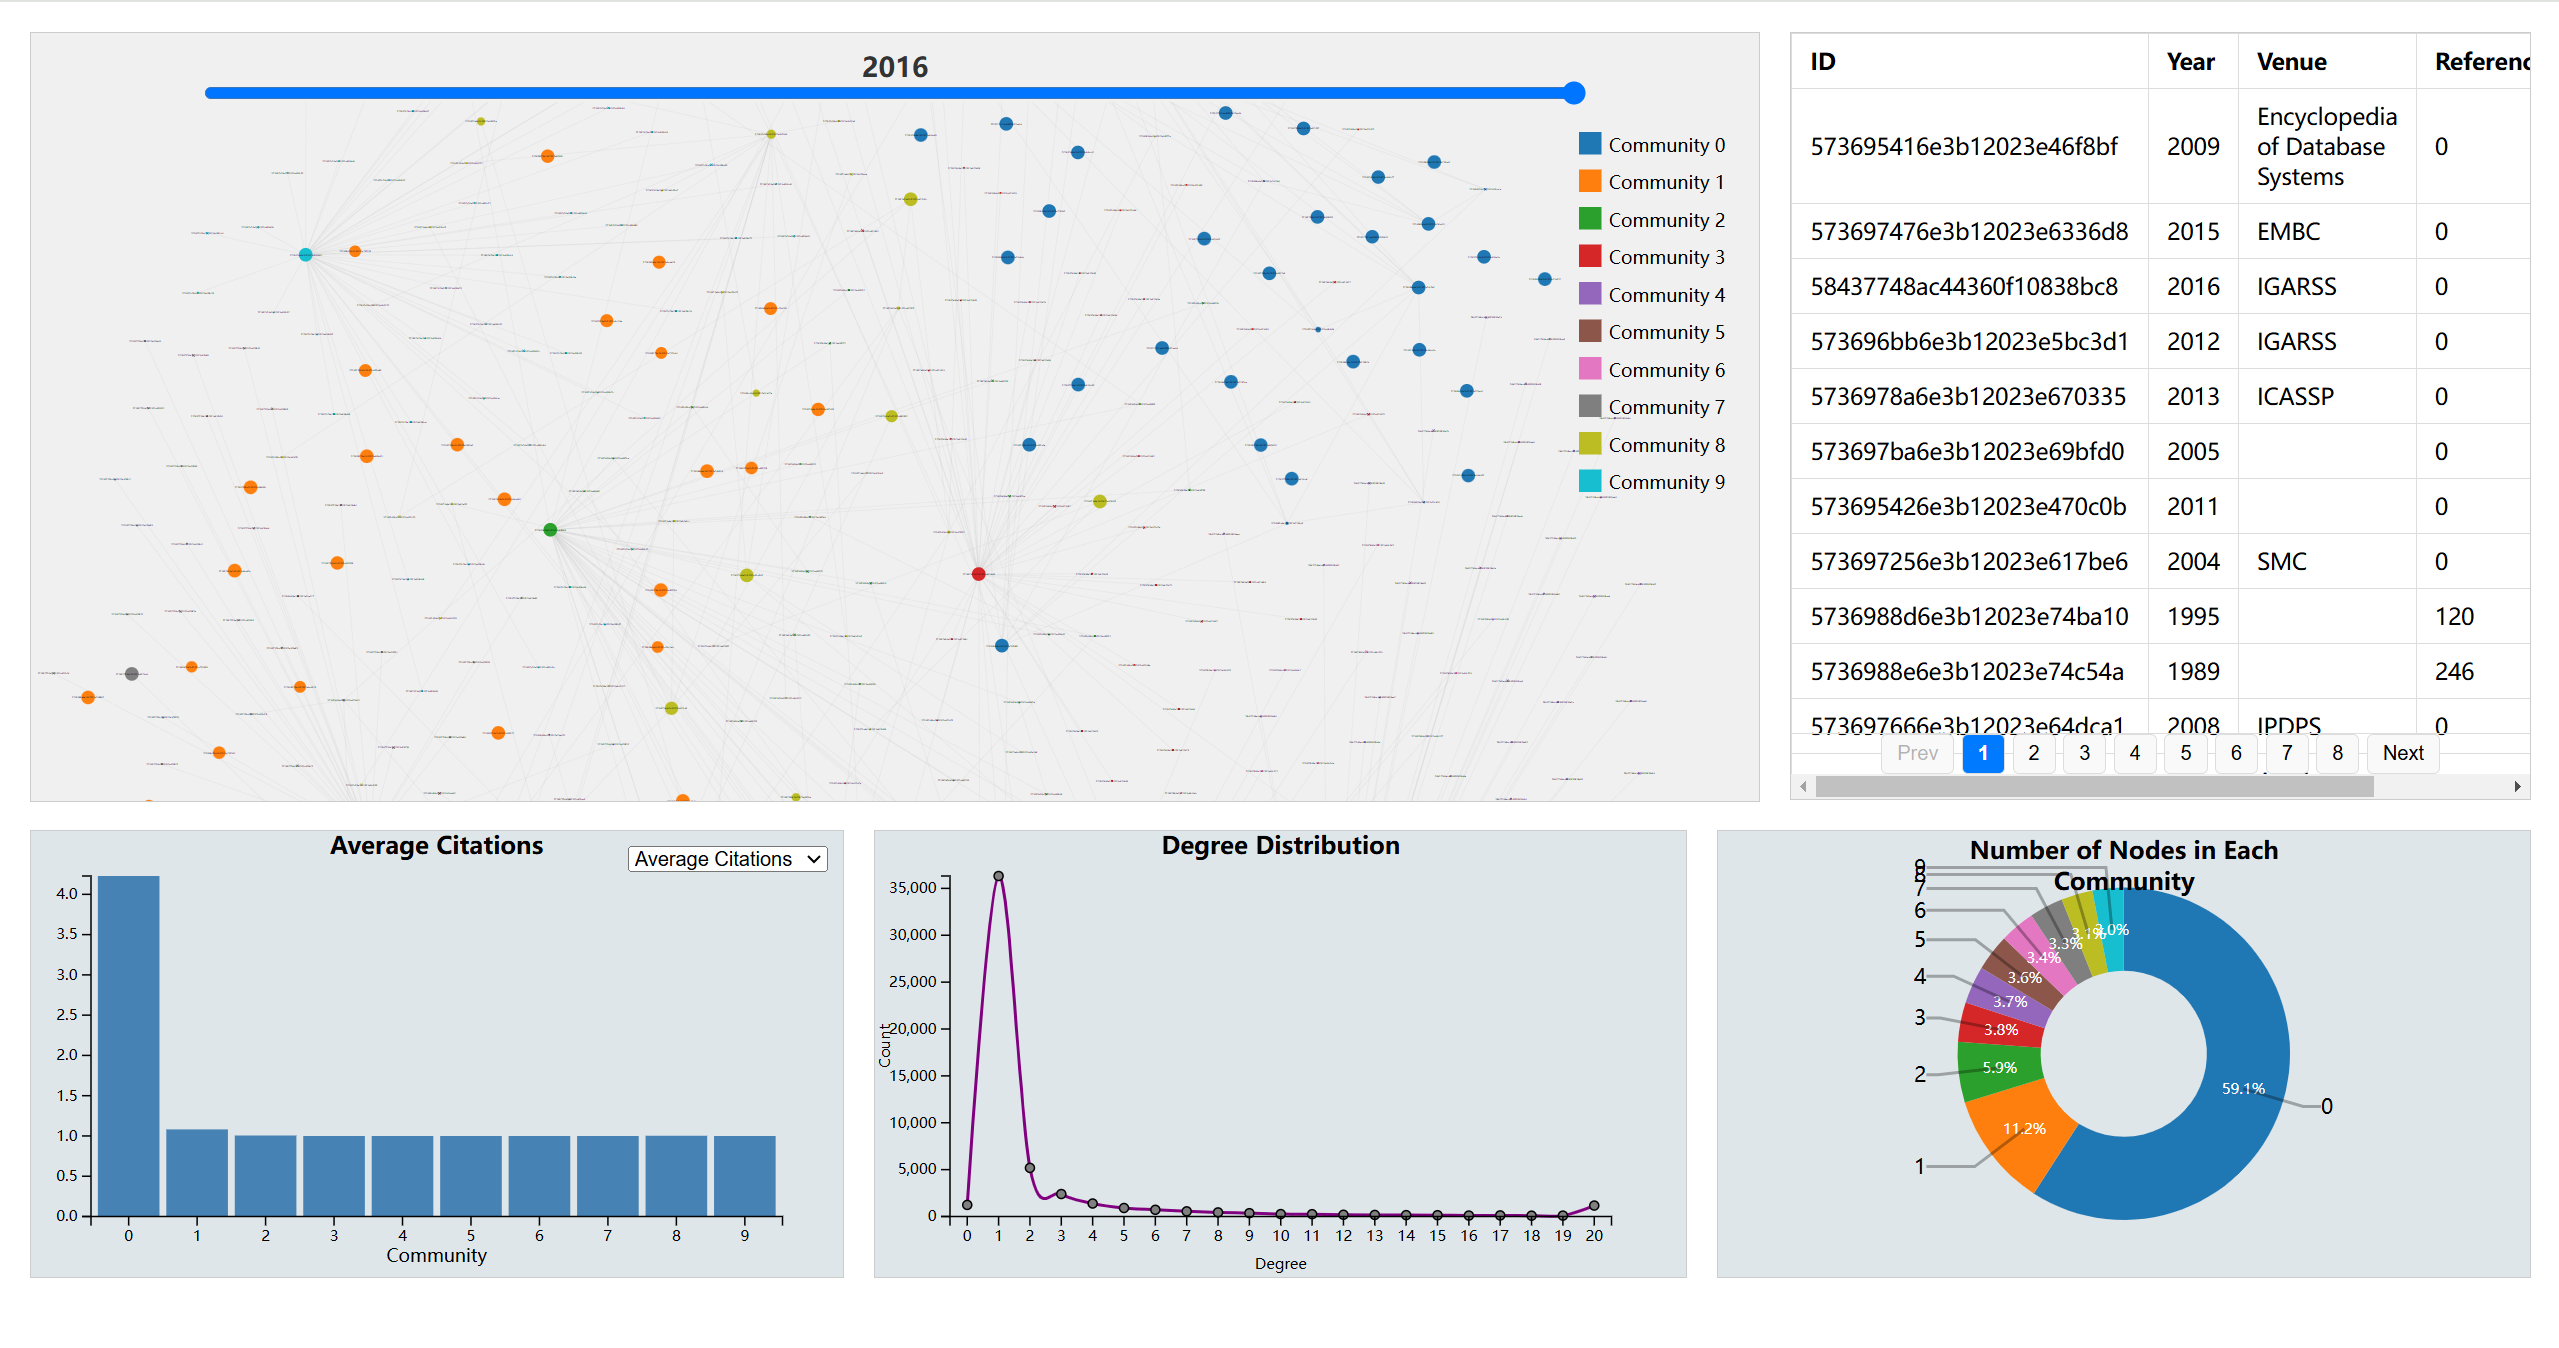
\includegraphics[width=0.48\textwidth]{img/introduction/visualization.png}
	\caption{Snapshot of the visualization system}
	\label{fig:visua}
\end{figure}

The subsequent sections of this report follow the analytical framework outlined below:
\\

\textbf{Preprocessing}: Transforming the raw DBLP data into a structured network through cleaning, filtering, and attribute assignment.

\textbf{Community Detection}: Identifying cohesive subgroups using algorithms like Louvain and Label Propagation to uncover collaboration dynamics and research specializations.

\textbf{Centrality Analysis}: Analyzing metrics such as degree centrality and PageRank to identify influential nodes and assess network topology.
\textbf{Link Prediction}: Employing the GLACE model on the Cora-ML dataset to predict future connections based on structural features, providing insights into evolving citation trends.

\textbf{Visualization}: Presenting findings through an interactive system developed with \textbf{Python} and \textbf{D3.js}, highlighting key network characteristics and community structures.
\\

This structured approach provides a comprehensive examination of the DBLP co-authorship and publication network, delivering insights into collaboration patterns, influential figures, and the evolution of academic networks.



\section{Preprocessing}

The preprocessing phase is a critical step in transforming the raw DBLP V9 dataset into a structured format suitable for detailed analysis. This stage encompasses data cleaning, network construction, feature engineering, and dataset filtering. The DBLP V9 dataset was specifically chosen for its balance between computational feasibility and data comprehensiveness, enabling robust analysis of academic collaboration and citation patterns within computer science.

\subsection{Dataset Selection}

The DBLP-Citation-network V9 dataset was selected due to its optimal balance between data richness and computational manageability, as summarized in Table \ref{tab:dblp_citation_networks}. Other versions of the DBLP dataset, while valuable, either lacked the depth of information or exceeded practical computational limits for this project. DBLP V9 captures key trends up to July 3, 2017, offering a comprehensive yet tractable dataset with \textbf{3,680,007 papers} and \textbf{1,876,067 citation relationships}.

\begin{table*}[h!]
	\centering
	\begin{tabular}{|c|c|c|}
		\hline
		\textbf{Dataset Version}          & \textbf{Number of Papers} & \textbf{Number of Citation Relationships} \\ \hline
		Citation-network V1               & 629,814                   & >632,752                                  \\ \hline
		Citation-network V2               & 1,397,240                 & >3,021,489                                \\ \hline
		DBLP-Citation-network V3          & 1,632,442                 & >2,327,450                                \\ \hline
		DBLP-Citation-network V4          & 1,511,035                 & 2,084,019                                 \\ \hline
		DBLP-Citation-network V5          & 1,572,277                 & 2,084,019                                 \\ \hline
		DBLP-Citation-network V6          & 2,084,055                 & 2,244,018                                 \\ \hline
		DBLP-Citation-network V7          & 2,244,021                 & 4,354,534                                 \\ \hline
		DBLP-Citation-network V8          & 3,272,991                 & 8,466,859                                 \\ \hline
		\textbf{DBLP-Citation-network V9} & \textbf{3,680,007}        & \textbf{1,876,067}                        \\ \hline
		DBLP-Citation-network V10         & 3,079,007                 & 25,166,994                                \\ \hline
		DBLP-Citation-network V11         & 4,107,340                 & 36,624,464                                \\ \hline
		DBLP-Citation-network V12         & 4,894,081                 & 45,564,149                                \\ \hline
		DBLP-Citation-network V13         & 5,354,309                 & 48,227,950                                \\ \hline
		DBLP-Citation-network V14         & 5,259,858                 & 36,630,661                                \\ \hline
	\end{tabular}
	\caption{Summary of DBLP Citation Network Versions}
	\label{tab:dblp_citation_networks}
\end{table*}

\subsection{Data Cleaning and Integration}

The raw DBLP dataset includes metadata such as titles, authors, venues, and citations. Data cleaning involved:
\begin{itemize}
	\item \textbf{Grouping Records:} Papers were grouped using unique identifiers to ensure each record was correctly structured.
	\item \textbf{Resolving Missing Data:} Missing fields, such as titles, authors, or venues, were assigned default values to maintain consistency.
\end{itemize}

These steps ensured the dataset was standardized and ready for subsequent analysis.

\subsection{Network Construction}

The dataset was represented as two interconnected networks:

\begin{enumerate}
	\item \textbf{Co-authorship Network:} In this network, authors are represented as nodes, with weighted edges denoting co-authorship relationships. The weight of each edge corresponds to the frequency of collaborations between authors. This network contains a total of 3,680,007 nodes (authors) and 1,876,067 edges (co-authorship relationships).

	\item \textbf{Citation Network:} The citation network is constructed by representing papers as nodes, with directed edges indicating citation relationships between them. Each edge direction signifies the citing paper and the cited paper. This network also comprises 3,680,007 nodes (papers) and 1,876,067 edges (citation relationships).
\end{enumerate}


This dual representation allows for a comprehensive study of collaboration and citation dynamics.

\subsection{Feature Engineering}

Key features were engineered to enhance the dataset’s analytical capabilities:
\begin{itemize}
	\item \textbf{Co-authorship Features:} Unique author identifiers were assigned, and collaboration frequencies were calculated.
	\item \textbf{Citation Metrics:} In-degree (citations received) and out-degree (references) were computed for each paper.
	\item \textbf{Venue Indexing:} Publication venues were standardized and indexed for uniform representation.
\end{itemize}

\subsection{Dataset Filtering}

Papers with no citations and references were flagged as "isolate" and excluded to improve computational efficiency. Additionally, thresholds were applied to focus on significant collaborations and impactful papers.

\subsection{Exploratory Analysis}

Exploratory analyses were conducted using Python libraries such as \texttt{pandas} and \texttt{matplotlib}. The key findings are visualized in Figures \ref{fig:num_authors_per_paper}--\ref{fig:num_coauthors_per_author}:

\begin{itemize}
	\item \textbf{Authors per Paper:} Most papers have few authors, with fewer multi-author publications.
	\item \textbf{Citation Distribution:} Citations are highly skewed, with a small number of papers receiving the majority of citations.
	\item \textbf{References per Paper:} Papers with more citations tend to reference more works.
	\item \textbf{Co-authors per Author:} A small group of authors collaborate extensively, while most have limited collaborations.
\end{itemize}

\begin{figure*}[htbp]
	\centering
	\begin{minipage}{0.24\textwidth}
		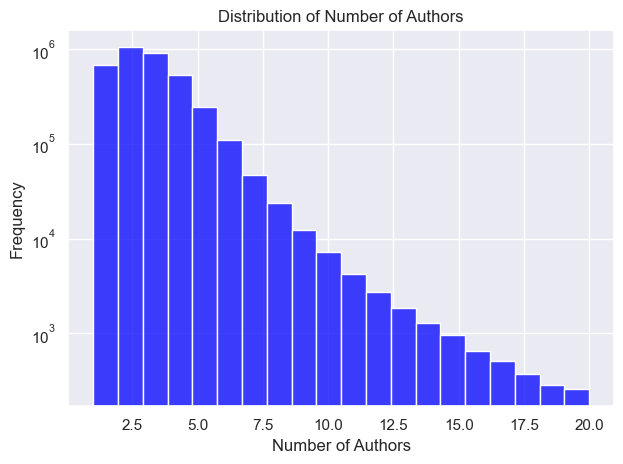
\includegraphics[width=\textwidth]{img/preprocess/num_authors.png}
		\caption{Number of Authors per Paper}
		\label{fig:num_authors_per_paper}
	\end{minipage} \hfill
	\begin{minipage}{0.24\textwidth}
		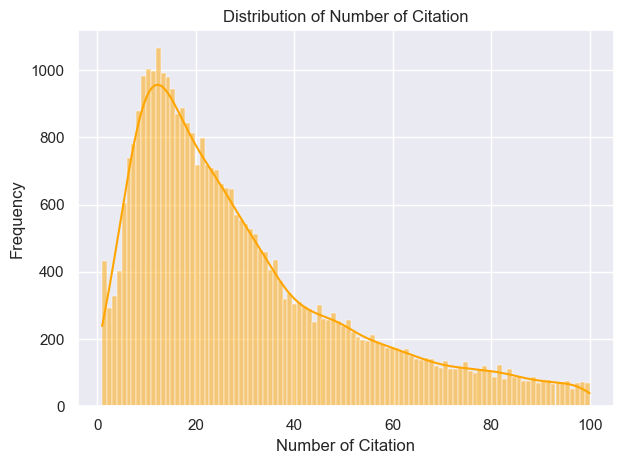
\includegraphics[width=\textwidth]{img/preprocess/num_citations.png}
		\caption{Citation Distribution of Papers}
		\label{fig:citation_distribution}
	\end{minipage} \hfill
	\begin{minipage}{0.24\textwidth}
		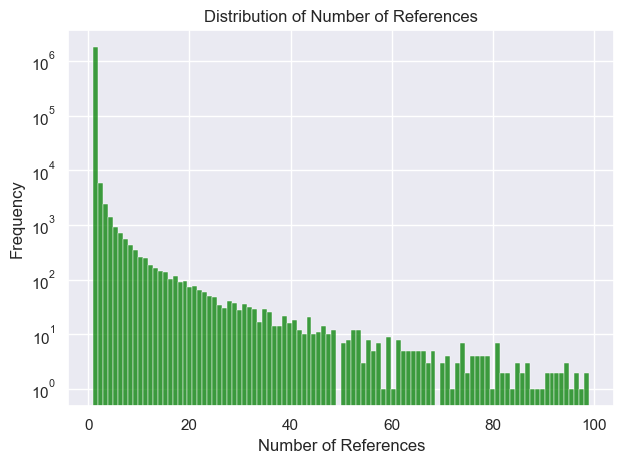
\includegraphics[width=\textwidth]{img/preprocess/num_references.png}
		\caption{Reference Distribution of Papers}
		\label{fig:reference_distribution}
	\end{minipage} \hfill
	\begin{minipage}{0.24\textwidth}
		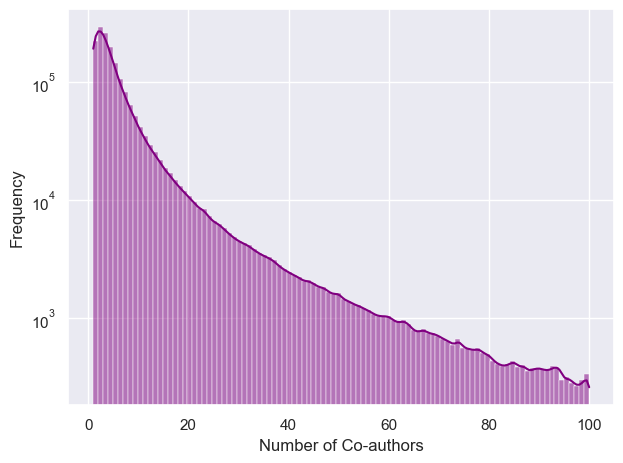
\includegraphics[width=\textwidth]{img/preprocess/num_coauthors.png}
		\caption{Number of Co-authors per Author}
		\label{fig:num_coauthors_per_author}
	\end{minipage}
\end{figure*}

These analyses offer critical insights into academic collaboration and citation patterns, laying the groundwork for deeper exploration of academic network structures.



\section{Community Mining}
In academic networks, community mining aims to identify cohesive subgroups reflecting collaborative dynamics, research specializations, and the structural foundation of scholarly interactions. Three common algorithms - Louvain, Label Propagation, and Multi - level - are used to discover potential communities based on node relationships.

After detection, community proportions and modularity are calculated to assess the quality of community division. They provide insights into the network's structure, indicating whether detected communities have strong internal and weak external connections, characteristic of well - formed community structures.

\subsection{Overview of Community Mining}
Community detections operate by grouping nodes in a graph based on their connectivity. In the context of academic networks, nodes represent entities such as papers or authors, and edges represent relationships between these entities, such as co-authorship or citations. Below are the specifics of Paper Networks and Author Networks.
\begin{itemize}
	\item {Paper Network:}In a paper network, nodes represent individual papers, and edges represent relationships such as citations or co-authorships. Edges are weighted by the number of citations or co-authors shared. Community detection aims to identify research areas or subfields where papers are closely linked by citations or co-authors, revealing thematic connections or shared academic topics.
	\item {Author Network:}In an author network, nodes represent authors, and edges represent co-authorships. The edge weight reflects the number of joint papers between authors, with higher weights indicating stronger collaboration. Community detection in this network uncovers collaborative groups or research teams, offering insights into research partnerships and collaboration patterns.
\end{itemize}

The goal of community detection is to find subsets of nodes (communities) where the internal connectivity is higher than expected by random chance, and the external connectivity is relatively lower. Mathematically, this is often expressed in terms of modularity.


\subsection{Community Detection Algorithms}

\subsubsection{Louvain Algorithm}
The Louvain algorithm is a method for detecting communities by optimizing modularity.
The modularity \( Q \) for a community division is calculated as:

\[
	Q = \frac{1}{2m} \sum_{i,j} \left( A_{ij} - \frac{k_i k_j}{2m} \right) \delta(c_i, c_j)
\]
Where:
\( m \) is the total number of edges in the network.
\( A_{ij} \) is the weight of the edge between nodes \( i \) and \( j \).
\( k_i \) and \( k_j \) are the degrees of nodes \( i \) and \( j \).
\( \delta(c_i, c_j) \) is 1 if nodes \( i \) and \( j \) are in the same community and 0 otherwise.
\( c_i \) and \( c_j \) are the community labels of nodes \( i \) and \( j \).

The Louvain algorithm works in two phases:

1. Local optimization: Each node is assigned to the community of its neighbor that maximizes modularity.

2. Community aggregation: Communities are treated as super-nodes, and the algorithm repeats the process of modularity optimization on this new, aggregated graph.

The algorithm is computationally efficient and is well-suited for large-scale networks, making it a popular choice in detecting academic collaboration communities.

\subsubsection{Label Propagation Algorithm}
Label Propagation (LP) is a simple and efficient algorithm where each node is initially assigned a unique label. At each iteration, each node updates its label to the most frequent label among its neighbors. This process continues until the labels stabilize.

Mathematically, Label Propagation is expressed as:

\[
	l_i^{(t+1)} = \arg\max_{l_j \in N(i)} \sum_{k \in N(i), l_k = l_j} \frac{1}{d_k}
\]
Where:
\( l_i^{(t+1)} \) is the new label for node
\( i \) after iteration \( t \). \( N(i) \) is the set of neighbors of node \( i \).
\( d_k \) is the degree of neighbor \( k \).

The algorithm is highly parallelizable and does not require predefined parameters like the number of communities. It is particularly efficient for large networks with many nodes and edges.

\subsubsection{Multi-level Algorithm}
The Multi-level algorithm is based on a hierarchical approach, where the graph is coarsened into a smaller graph by iteratively merging nodes that are highly connected. The algorithm detects communities at multiple levels by optimizing modularity at each level. After the graph is coarsened, the community detection process is applied to the smaller graph, and the solution is refined by uncoarsing the graph back to its original size.

The Multi-level algorithm follows these general steps:

1. Coarsing: Repeatedly reduce the graph by merging highly connected nodes, creating a smaller graph at each level.

2. Community Detection: Perform community detection on the coarsed graph (typically using modularity maximization).

3. Uncoarsing: Refine the community structure by uncoarsing the graph and applying the community structure from the coarser level to the finer levels.

This method can efficiently handle large-scale networks and is suitable for discovering communities at different scales.

\subsubsection{Reasons for Choosing These Algorithms}
These three algorithms represent different approaches to community detection:
\begin{itemize}
	\item Louvain emphasizes modularity optimization and is efficient for large networks.
	\item Label Propagation uses local information propagation and is highly scalable and efficient.
	\item Multi-level works at multiple scales, ensuring that communities are detected at both coarse and fine levels.
\end{itemize}

Each algorithm brings unique strengths, making them well-suited for the diverse and complex academic networks that we are analyzing.


\subsection{Community Proportions}
The community proportions represent the distribution of nodes across different communities. By calculating the size of each community (i.e., the number of nodes within it) and dividing by the total number of nodes, we can get the proportion of each community in the overall network.

Let \( N_c \) be the number of nodes in community \( c \), and $ N_{\text{total}} $ be the total number of nodes in the network. The proportion of community \( c \) is given by:

\begin{equation}
	\text{Proportion of community } c = \frac{N_c}{N_{\text{total}}}
	\nonumber
\end{equation}

This helps to understand the size and importance of each community within the entire network. Larger communities may represent more significant areas of academic collaboration, while smaller ones could represent more specialized or niche research areas.

\subsection{Modularity}

Modularity is a key measure used to evaluate the quality of community detection. It quantifies the strength of division of a network into communities by comparing the number of edges within communities to the number of edges expected by random chance.

The modularity \( Q \) is calculated using the formula mentioned earlier. A modularity value greater than 0 indicates that the community division is better than a random distribution of edges, with higher values indicating stronger community structures.

A common threshold is:

\( Q > 0.7 \): A good community structure.

\( Q < 0.7 \): A poor division, where the community structure is weaker than random.



\section{Centrality Measurement}

After detecting communities within the academic network, it is essential to assess the importance and influence of individual nodes within each community. In this analysis, centrality measures such as Degree Centrality and PageRank Centrality were calculated to identify influential nodes, revealing key hubs and authoritative figures within the network. Additionally, structural characteristics of the network, including community diameters and average citations per author, were analyzed to understand the overall network topology and functional properties. The following sections describe the methodology and results of these calculations:

\subsection{Centrality Calculation}

\subsubsection{Degree Centrality}

This measure counts the number of direct connections (edges) a node has, reflecting its immediate popularity or connectivity within the network. A higher degree centrality indicates a node that is well-connected, potentially influencing many other nodes within the community. Degree centrality is particularly useful for identifying the most central or influential nodes based on direct relationships.

The degree centrality \( C_d(i) \) for a node \( i \) is calculated as:

\[
	C_d(i) = \text{deg}(i)
\]
Where \( \text{deg}(i) \) is the number of edges connected to node \( i \).

\subsubsection{PageRank Centrality}

PageRank, developed by Google to rank web pages, measures the influence of a node by considering both the number and quality (weight) of its incoming edges. In the context of academic networks, PageRank helps identify authoritative nodes, where a high PageRank centrality indicates that a node is not only well-connected but also highly regarded by other influential nodes.

PageRank centrality \( PR(i) \) for node \( i \) is computed iteratively based on the network structure:

\[
	PR(i) = \frac{1 - d}{N} + d \sum_{j \in \mathcal{N}(i)} \frac{PR(j)}{|\mathcal{N}(j)|}
\]
Where:
\( d \) is the damping factor (usually set to 0.85),
\( N \) is the total number of nodes in the network,
\( \mathcal{N}(i) \) is the set of neighbors of node \( i \),
\( |\mathcal{N}(j)| \) is the number of outgoing edges from node \( j \).

\subsubsection{Why Degree Centrality and PageRank Centrality?}

The selection of Degree Centrality and PageRank Centrality as centrality measures is based on their ability to capture different yet complementary aspects of node influence and importance within a network.

\begin{itemize}
	\item Degree Centrality measures the number of direct connections a node has. In academic networks, it identifies the most connected authors or papers, making it useful for spotting collaboration hubs and active contributors.
	\item PageRank Centrality considers both the number and quality of connections, giving more importance to nodes linked to influential ones. This helps identify authoritative figures and key players in the network.
\end{itemize}

Together, these measures provide a well-rounded view of node influence, capturing both direct connectivity (Degree) and overall importance (PageRank).


\subsection{Community Diameters}

The diameter of a community refers to the longest shortest path between any two nodes within that community. A smaller diameter indicates that nodes within the community are relatively close to one another, suggesting a more cohesive community. In contrast, a larger diameter may indicate the presence of disconnected subgroups or more sparse relationships between community members.




\section{Link Prediction}

\section{Visualization System}

\section{Conclusion}

\section*{Acknowledgements}


% % Entries for the entire Anthology, followed by custom entries
% \bibliography{anthology,custom}
% \bibliographystyle{acl_natbib}

% \appendix

% \section{Example Appendix}
% \label{sec:appendix}

% This is a section in the appendix.

\end{document}
